\section{Systemdesign}

% TODO: Flytta rubrikerna till rätt filer. 

\subsection{Problembeskrivning}
Detta är en enkel beskrivning på vårt koncept om hur programmet ska fungera. Man har ett konvext kvadratiskt minimeringsproblem som man vill lösa. Problemet skickas till vårt program som med effektiva algoritmer utvalda av oss räknar ut den optimala lösningen \textit{z*}.

\begin{figure}[h]
	\begin{center}
		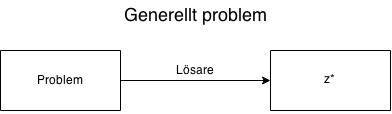
\includegraphics[scale=0.7]{bilder/Generellt.png}
	\end{center}
	\caption{Enkel beskrivning av problemet.}
\end{figure}

\subsection{Standarder}
Källkoden följer de standarder som är beskrivna i kvalitetsplanen.

\subsection{Systemskiss}
Programmet kommer i huvudsak köras via Matlab, där kommer programmet anropas som en funktion med all indata i parametrarna. Indatan kommer sedan kompileras till en header fil som sedan skickas till mex solvern. QP-solvern kommer sedan lösa problemet utifrån kompilerade datan och sedan returnera resultatet till matlab. Programmet kommer även att kunna köras från vårt eget GUI, där man i GUI:t kan mata in sitt QP problem och de matriser man vill använda, generera en C-problemfil som kan lösas av C solvern. Resultatet skickas sedan tillbaka och visas i GUI:t.

\begin{figure}[H]
	\begin{center}
		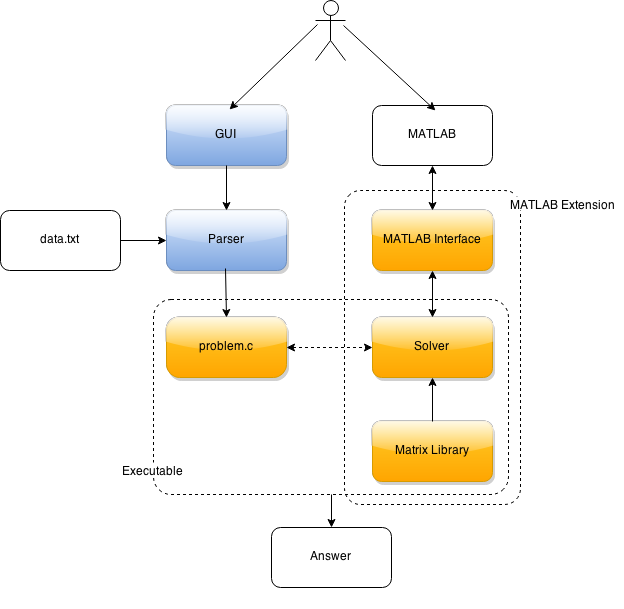
\includegraphics[scale=0.7]{bilder/arkitektur.png}
	\end{center}
	\caption{Övergripande beskrivning av systemet.}
\end{figure}

%% Graphic for TeX using PGF
% Title: C:\Users\sebfas\Pictures\Systemskiss.dia
% Creator: Dia v0.97.2
% CreationDate: Sun Feb 15 00:30:41 2015
% For: sebfas
% \usepackage{tikz}
% The following commands are not supported in PSTricks at present
% We define them conditionally, so when they are implemented,
% this pgf file will use them.
\ifx\du\undefined
  \newlength{\du}
\fi
\setlength{\du}{15\unitlength}
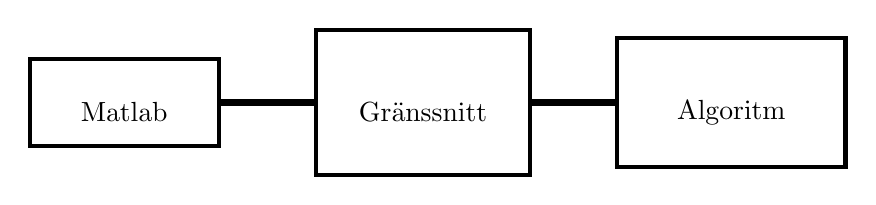
\begin{tikzpicture}
\pgftransformxscale{1.000000}
\pgftransformyscale{-1.000000}
\definecolor{dialinecolor}{rgb}{0.000000, 0.000000, 0.000000}
\pgfsetstrokecolor{dialinecolor}
\definecolor{dialinecolor}{rgb}{1.000000, 1.000000, 1.000000}
\pgfsetfillcolor{dialinecolor}
\definecolor{dialinecolor}{rgb}{1.000000, 1.000000, 1.000000}
\pgfsetfillcolor{dialinecolor}
\fill (1.400000\du,1.700000\du)--(1.400000\du,3.800000\du)--(5.950000\du,3.800000\du)--(5.950000\du,1.700000\du)--cycle;
\pgfsetlinewidth{0.100000\du}
\pgfsetdash{}{0pt}
\pgfsetdash{}{0pt}
\pgfsetmiterjoin
\definecolor{dialinecolor}{rgb}{0.000000, 0.000000, 0.000000}
\pgfsetstrokecolor{dialinecolor}
\draw (1.400000\du,1.700000\du)--(1.400000\du,3.800000\du)--(5.950000\du,3.800000\du)--(5.950000\du,1.700000\du)--cycle;
% setfont left to latex
\definecolor{dialinecolor}{rgb}{0.000000, 0.000000, 0.000000}
\pgfsetstrokecolor{dialinecolor}
\node at (3.675000\du,2.990000\du){Matlab};
\definecolor{dialinecolor}{rgb}{1.000000, 1.000000, 1.000000}
\pgfsetfillcolor{dialinecolor}
\fill (8.300000\du,1.000000\du)--(8.300000\du,4.500000\du)--(13.450000\du,4.500000\du)--(13.450000\du,1.000000\du)--cycle;
\pgfsetlinewidth{0.100000\du}
\pgfsetdash{}{0pt}
\pgfsetdash{}{0pt}
\pgfsetmiterjoin
\definecolor{dialinecolor}{rgb}{0.000000, 0.000000, 0.000000}
\pgfsetstrokecolor{dialinecolor}
\draw (8.300000\du,1.000000\du)--(8.300000\du,4.500000\du)--(13.450000\du,4.500000\du)--(13.450000\du,1.000000\du)--cycle;
% setfont left to latex
\definecolor{dialinecolor}{rgb}{0.000000, 0.000000, 0.000000}
\pgfsetstrokecolor{dialinecolor}
\node at (10.875000\du,2.990000\du){Gränssnitt};
\definecolor{dialinecolor}{rgb}{1.000000, 1.000000, 1.000000}
\pgfsetfillcolor{dialinecolor}
\fill (15.550000\du,1.200000\du)--(15.550000\du,4.300000\du)--(21.050000\du,4.300000\du)--(21.050000\du,1.200000\du)--cycle;
\pgfsetlinewidth{0.100000\du}
\pgfsetdash{}{0pt}
\pgfsetdash{}{0pt}
\pgfsetmiterjoin
\definecolor{dialinecolor}{rgb}{0.000000, 0.000000, 0.000000}
\pgfsetstrokecolor{dialinecolor}
\draw (15.550000\du,1.200000\du)--(15.550000\du,4.300000\du)--(21.050000\du,4.300000\du)--(21.050000\du,1.200000\du)--cycle;
% setfont left to latex
\definecolor{dialinecolor}{rgb}{0.000000, 0.000000, 0.000000}
\pgfsetstrokecolor{dialinecolor}
\node at (18.300000\du,2.990000\du){Algoritm};
\pgfsetlinewidth{0.150000\du}
\pgfsetdash{}{0pt}
\pgfsetdash{}{0pt}
\pgfsetbuttcap
{
\definecolor{dialinecolor}{rgb}{0.000000, 0.000000, 0.000000}
\pgfsetfillcolor{dialinecolor}
% was here!!!
\definecolor{dialinecolor}{rgb}{0.000000, 0.000000, 0.000000}
\pgfsetstrokecolor{dialinecolor}
\draw (5.950000\du,2.750000\du)--(8.300000\du,2.750000\du);
}
\pgfsetlinewidth{0.150000\du}
\pgfsetdash{}{0pt}
\pgfsetdash{}{0pt}
\pgfsetbuttcap
{
\definecolor{dialinecolor}{rgb}{0.000000, 0.000000, 0.000000}
\pgfsetfillcolor{dialinecolor}
% was here!!!
\definecolor{dialinecolor}{rgb}{0.000000, 0.000000, 0.000000}
\pgfsetstrokecolor{dialinecolor}
\draw (13.450000\du,2.750000\du)--(15.550000\du,2.750000\du);
}
\end{tikzpicture}



%\subsection{Arkitekturens delar}
%Arkitekturen är uppdelad i tre större delar där GUI:t och parsern är en del
%Lösningsalgoritmen solvern är en del ... active-set-metoden
%Integrationen mot matlab är en del ... funktioner...

\subsection{Matrisbibliotek}
Arkitekturen innehåller ett eget matrisbibliotek, innehållande alla nödvändiga matrisoperationer för lösaren.

